\documentclass[a4paper,10pt]{scrreprt}

% GENERAL LATEX PACKAGES
\usepackage{subcaption}
\usepackage{graphicx}
\usepackage{color}
\usepackage{xcolor}
\usepackage{url}
\usepackage{hyperref}
\usepackage{mathtools}
\usepackage{wasysym}
\usepackage{lscape}
\usepackage{fancyvrb}

% TIKZ FOR NICE LATEX GRAPHICS
\usepackage{tikz}
\usetikzlibrary{shadows,arrows}
\usetikzlibrary{shapes.geometric}
\usetikzlibrary{shapes.symbols} 
\usetikzlibrary{decorations.shapes}
\usetikzlibrary{shapes.arrows}
\usepackage{styleimports/definitions} 		%some custom commands and math operators
\usepackage{styleimports/alica-tikz}		  %colours for ALICA plans etc.

% BIBLIOGRAPHY PACKAGE CONFIGURATION
\usepackage[
	backend=biber,
	citestyle=numeric-comp,
	bibstyle=numeric-comp,
	maxbibnames=10,
	maxcitenames=2,
	natbib=true,
	hyperref=true
]{biblatex}
\addbibresource{bibtex.bib}

% HYPERREF PACKAGE CONFIGURATION
\usepackage{hyperref}
\hypersetup{
	colorlinks,
	citecolor=black,
	filecolor=black,
	linkcolor=blue!60!black,
	urlcolor=blue!60!black,
	pdftitle = {Distributed Cooperative Robot Systems},
	pdfauthor = {Stephan Opfer},
	pdfkeywords = {Multi-Agent Systems, Knowledge Representation}
}

\title{Distributed Cooperative Robot Systems}
\author{Lecturers and Students}
\makeindex

% DOCUMENT BEGINS
\begin{document}

\maketitle
\tableofcontents

\chapter{Introduction}
\label{chap:Introduction}

\section{Purpose of this Document}
\label{sec:Purpose}

Instead of giving the students a lot of Powerpoint slides that compress the complex topics of this course into a bunch of bullet points, we wanted the students to have a dedicated document for preparing their exam. Unfortunately, such a document is a lot more work and it needs several iterations of thorough reviewing. Therefore, we came up with the compromise that the students write this document theirselves and the lecturers only have to review and improve it. 

Maybe you ask: "What is wrong with Powerpoint?" 

A Powerpoint presentation should aid a presenter in presenting a certain message or information to his audience. The slides alone often miss critical parts (that couldn't easily condensed into bullet points) and are unclear without the corresponding vocal line of the presenter. Nevertheless, students end up alone with the slides trying to prepare their examinations.

Apart from that, try to google topics like "disadvantages of powerpoint" or "why we should ban Powerpoint" and you will find interesting articles that connect Powerpoint and the Accident of the Columbia Space Shuttle [\href{http://www.nytimes.com/2003/12/14/magazine/2003-the-3rd-annual-year-in-ideas-powerpoint-makes-you-dumb.html}{1}] [\href{http://www.edwardtufte.com/bboard/q-and-a-fetch-msg?msg_id=0001yB&topic_id=1&topic=Ask+E%2eT%2e}{2}].

\section{How to Contribute to this Document?}
\label{sec:Contribute}

Basically there are two aspects. At first you need to get the \LaTeX\  source code of this document from our \href{https://github.com/carpe-noctem-cassel/cnc-turtlebots}{cnc-turtlebots GitHub Repository}. It is located in the folder \verb#doc/latex#. Anybody can download it, but for making changes to it you need to have an GitHub-Account which was given the corresponding privileges. That is typically arranged during the first session of this course. 

This leaves us with the requirements, that you are able to write \LaTeX\ and know how to use GIT in combination with GitHub. Regarding GIT and GitHub we recommend to read Section~\ref{sec:Git}. 

Maybe \LaTeX\ is hard to master when it comes to tables, graphics and customising the layout of a document, but you don't have to do that for contributing to this document. You should only be able to write text referencing images and place useful links from time to time. Furthermore, you should be able to structure the content into chapters, sections, and subsections. Everything just mentioned is already done in this document, so you can start by copying commands from the corresponding sections. 

For further reference and an in-depth study of \LaTeX, we recommend the following sources:

\begin{description}
  \item[\href{http://www.wiwiss.fu-berlin.de/fachbereich/vwl/iso/links/latex_einfuehrung_manuela_juergens.pdf}{\LaTeX\ \textendash\ eine Einf\"uhrung und ein bisschen mehr}:] A little bit longer introduction to \LaTeX\ basics.
  \item[\href{https://en.wikibooks.org/wiki/LaTeX}{\LaTeX\ WikiBook}:] Nice for looking up simple stuff. 
  \item[\href{https://tex.stackexchange.com}{tex.stackexchange.com}:] Stack Overflow for \LaTeX
  \item[\href{http://ftp.fau.de/ctan/graphics/pgf/base/doc/pgfmanual.pdf}{TikZ}:] \LaTeX package for designing advanced graphics directly in \LaTeX.
\end{description}

The final issue is to decide which editor you choose for compiling this \LaTeX document. We recommend \href{http://www.xm1math.net/texmaker/}{TexMaker}, because it is available for Ubuntu and Windows, although, there currently exists an issue with short cuts under Ubuntu 16.04 LTS. Consider this \href{http://askubuntu.com/questions/786280/texmaker-shortcuts-not-working-on-ubuntu-16-04}{Ask Ubuntu Post} for solving it.

With TexMaker you only have to open the \verb#Software_Reference_Book.tex# file and click on \verb#Quick Build#. If you get compile errors, you probably need to install the necessary \LaTeX packages. Under Ubuntu this is done by executing the following console command:

\verb#sudo apt-get install texlive-full#


\chapter{Foundations}
\label{chap:foundations}

In this chapter topics that are tackled during the lecture are introduced in a basic fashion. This includes agents, sensor, actuators, communication, etc\dots

\section{Agents}
\label{sec:agents}

Although not every agent is autonomous, our focus in this lecture is to design autonomous agents. Autonomous means, that the agent is not controlled from some external entity. It only perceives its environment and acts in order to change it. Why it tries to change its environment depends on the agent's properties. Agents can be reactive or proactive, they can communicate with other agents, remember the history of the environment, and predict the future of the environment according to some model. As a designer of the agents, you need to decide what kind of agents you need to achieve your goal. The famous book \emph{Artificial Intelligence \textendash\ A Modern Approach}, written by Russel and Norvic, elaborates properties of agents and environment in chapter two. The book is available in our library. It is recommended to read chapter two for your exam preparations.

\subsection{Robot Control Architectures}
\label{ssec:robotcontrolarch}

\begin{figure}[htbp]
  \centering
  \begin{tikzpicture}[every node/.append style={thick}]
    \node(Agent)[plan, minimum width=2.5cm] at (0,0) {Agent};
    \node(Environment) [plan, minimum width=2.5cm] at (0,-1) {Environment};
    \draw[->, bend left] (Agent.south east) to node[right] {act} (Environment.north east);
    \draw[->, bend left] (Environment.north west) to node[left] {perceive} (Agent.south west);
  \end{tikzpicture}
  \caption{Simple Control Loop}
  \label{fig:simplecontrolloop}
\end{figure}

Usually it is believed that the agent is interacting with its environment \textendash whatever that environment is. This relation is often depicted as an agent-environment cycle (see Figure~\ref{fig:simplecontrolloop}). As mentioned before, the details of an agent architecture do vary from use case to use case.

\begin{figure}[htbp]
  \centering
  \begin{tikzpicture}[every node/.append style={thick}]
    
    \node(Data) at (0,0) {Data Layers};
    \node(SymbolLayer)[highLayer, anchor=north] at (Data.south) {};
    \node(SymbolLayerText)[anchor=north west] at (SymbolLayer.north west) {\tiny{\textbf{Symbol Layer}}};
    \node(SymbolLayerData)[data] at (SymbolLayer.south west) {\tiny{\textbf{Data:}\\[0.5em]Symbols, Rules,\\ Relations}};

    \node(IntermediateLayer)[midLayer, anchor=north west] at (SymbolLayer.south west) {};
    \node(IntermediateLayerText)[anchor=north west] at (IntermediateLayer.north west) {\tiny{\textbf{Intermediate Layer}}};
    \node(IntermediateLayerData)[data] at (IntermediateLayer.south west) {\tiny{\textbf{Data:}\\[0.5em]Feature Vectors, Raw Map}};

    \node(SensorimotorLayer)[lowLayer, anchor=north west] at (IntermediateLayer.south west) {};
    \node(SensorimotorLayerText)[anchor=north west] at (SensorimotorLayer.north west) {\tiny{\textbf{Sensorimotor Layer}}};
    \node(SensorimotorLayerData)[data] at (SensorimotorLayer.south west) {\tiny{\textbf{Data:}\\[0.5em]Raw Data}};

    \node(ButtomUp)[single arrow, shape border rotate=90, draw, anchor=center, minimum height=5.02cm, xshift=-1cm, text width=1cm, align=center] at (IntermediateLayer.west) {\tiny{Data Abstraction}};
    \draw[->, bend right] (IntermediateLayerData.east) to node [processingArrow] {\tiny{Symbol\\Grounding,\\Anchoring}} (SymbolLayerData.south east);
    \draw[->, bend right] (SensorimotorLayerData.east) to node [processingArrow] {\tiny{Smoothing,\\ Filtering}} (IntermediateLayerData.south east);

    \node(Processing) at (6,0) {Control Layers};
    \node(DeliberateLayer)[highLayer, anchor=north] at (Processing.south) {};
    \node(DeliberateLayerText)[anchor=north west] at (DeliberateLayer.north west) {\tiny{\textbf{Deliberation Layer}}};
    \node(DeliberateLayerData)[data] at (DeliberateLayer.south west) {\tiny{\textbf{Control:}\\[0.5em]Communication, Planning, Strategy Evaluation}};

    \node(SequencerLayer)[midLayer, anchor=north west] at (DeliberateLayer.south west) {};
    \node(SequencerLayerText)[anchor=north west] at (SequencerLayer.north west) {\tiny{\textbf{Sequencer Layer}}};
    \node(SequencerLayerData)[data] at (SequencerLayer.south west) {\tiny{\textbf{Control:}\\[0.5em]Path Planning, Strategy}};

    \node(ControlLayer)[lowLayer, anchor=north west] at (SequencerLayer.south west) {};
    \node(ControlLayerText)[anchor=north west] at (ControlLayer.north west) {\tiny\textbf{{Reactive Control Layer}}};
    \node(ControlLayerData)[data] at (ControlLayer.south west) {\tiny{\textbf{Control:}\\[0.5em]Reaction,\\Controlling}};
    
    \node(TopDown)[single arrow, shape border rotate=270, draw, anchor=center, minimum height=5.02cm, xshift=+1cm, text width=1cm, align=center] at (SequencerLayer.east) {\tiny{Decision Making and Execution}};
    \draw[<-, bend left] (SequencerLayerData.west) to node [processingArrow, text width=1cm, left, yshift=2mm] {\tiny{Strategy\\Adaption}} (DeliberateLayerData.south west);
    \draw[<-, bend left] (ControlLayerData.west) to node [processingArrow, text width=1.1cm, left, yshift=2mm] {\tiny{Behaviour\\Adaption}} (SequencerLayerData.south west);
    
    \node(Environment) [minimum width=9cm, minimum height=0.8cm, draw=black!85] at (3,-7) {Environment};
    \draw[->, bend right] (ControlLayerData.west) to node [left] {\tiny{act}} ([xshift=1.3cm]Environment.north);
    \draw[->, bend right] ([xshift=-1.8cm]Environment.north) to node [right] {\tiny{sense}} (SensorimotorLayerData.east);
    
    \draw[<->] ([yshift=5mm]SymbolLayer.east) to ([yshift=5mm]DeliberateLayer.west);
    \draw[<->] ([yshift=-5mm]IntermediateLayer.east) to ([yshift=-5mm]SequencerLayer.west);
    \draw[<->] (SensorimotorLayer.east) to (ControlLayer.west);
  \end{tikzpicture}
  \caption{Control Loop}
  \label{fig:controlloop}
\end{figure}

In Figure~\ref{fig:controlloop} an overview of the details of a state-of-the-art robot control system is shown. You should consider a robot as a physical agent, i.d., an agent with a physical representation. The Data Layers on the left hand side represent the utilised algorithms to gain information and knowledge from raw sensor data. During the data processing, the data is continuously filtered, condensed, and abstracted until symbols and relations can be integrated into a symbolic knowledge representation. This knowledge is required by the algorithms on the right hand side of Figure~\ref{fig:controlloop}. The Deliberation Layer, including algorithms for planning, communication, and strategy evaluation, computes its decisions based on the knowledge of the symbolic knowledge representation. The results are processed by the Sequencer Layer and transformed into commands for controlling actuators of the robot. 
 
The data abstraction and decision making cycle is not perfectly followed in all applications. Often the abstraction of data up to the level of symbols and relations is not necessary. Moreover, it isn't clever to make everything a decision on the top most available layers. Think of a robot control architecture as of a human brain. A lot of things in a human body are handled without having the brain actively thinking about it, e.g., breathing, heart beat, reflexes on your knee, sneezing, blinking, etc. For a robot the corresponding things could be obstacle avoidance, motor controlling, avoiding rough terrain such as stairs, etc. Things like that should also in a robot control architecture be handled on lower levels and not bothering algorithms for planning or communication. 
 
However, don't take this easy. It can be quit difficult or even impossible to assign a certain task to a certain level. Obstacle avoidance, for example, is sometimes part of all three layers: While driving along a path, the robot in a office environment avoids humans or other robots by directly reacting to its 2D distance scans from its laser scanner (lower layers). The path itself is planned in order to avoid already known walls and finding the shortest path (intermediate layers). Planning this path is influenced by some knowledge about the environment, e.g., the robot knows that there is currently a meeting going on in some room and as the robots motion is relative noisy, it knows that it should avoid meetings like a virtual obstacle, in order to not disturb the meeting (top layers).

If you are in the position to decide on which layer something should be implemented, it sometimes helps to think about the following. The effort for abstracting data rises with each necessary processing step, therefore creating symbolic knowledge is often very costly. On the one hand, this argues for putting everything as on the lowest levels. On the other hand, the data on the lowest levels is often very large in terms of memory. You often have to ponder, whether it is more efficient to abstract the data and thereby reduce it to the smallest possible size or whether it is more efficient to directly operate on millions of raw camera pixel values without explicitly representing objects in the environment. Sometimes technical limitations also force you to a certain direction. If your robots, for example, need to communicate about objects it is probably impossible to send whole images of the objects to each other due to bandwidth limitations. Instead, the objects have to be abstracted to symbols or coordinates in order to match the bandwidth restrictions.

\section{Sensors}
\label{sec:sensor}

Sensors are the only option for an agent to perceive its environment. This also means, that everything that helps an agent to perceive its environment can be considered as a sensor. Nevertheless, sensors are also used to measure internal values, not belonging to the environment. Before we are going to deep, let us start the sensor topic a little bit more general. There are two sensor properties that help to categorise the plethora of sensors available nowadays: Active vs. passive sensors and external vs. internal sensors. Whether a sensor is active or passive determines the way it measures some value.

\begin{description}
 \item [active:] An active sensor emits something, e.g., energy, for measuring what ever it should measure. Typical examples are laser scanners or radars that emit electro-magnetic waves of different wave length.
 \item [passive:] Passive sensors directly measure energy from the environment. A camera for example perceives sunlight that is reflected from a surface, furthermore a compass measures the terrestrial magnetic field.
\end{description}

The difference between an internal or external sensor are the type of values the sensor measures, not how it measures it.
 
\begin{description}
 \item [internal:] Internal sensors measure values that are part of the system itself. Therefore it depends on the borders between the system and its environment. In case of a robot an internal sensor value could be its battery levels.
 \item [external:] External sensors measure values from the outside of the system, i.d., values from its environment. Typical values are distances, light, and sound.
\end{description}


\section{Actuators}
\label{sec:actuators}

\section{Communication}
\label{sec:communication}

\chapter{External Software and Developing Tools}
\label{chap:ExtSoftware}

This chapter is intended to give a short introduction to external software packages or frameworks, we utilise for the Carpe Noctem Cassel software framework.

\section{GIT and GitHub}
\label{sec:Git}

GIT is one of the most advanced version control systems currently available. Nevertheless, during our daily work we only use 20\% of its functionality. So for starters try to learn the stuff you need and ignore its advanced features like \emph{rebase} and \emph{cherry pick}.

The best reference and documentation about GIT can be found at \url{http://www.git-scm.com/docs}

Most of our software is published open source under the MIT License at our \href{https://github.com/dasys-lab}{GitHub Repositories}. Therefore, it is also interesting to read about the features of GitHub, like SSH-Key based authorization, groups, organisations, and MarkDown.

The README.md files in our repositories are written in \href{https://en.wikipedia.org/wiki/Markdown}{MarkDown}, because GitHub parses these MarkDown files and auto-generates an HTML documentation from it.

A list of GIT commands, that should be enough for the start, can be found on \href{https://www.git-tower.com/blog/git-cheat-sheet/}{git-tower.com}.

\section{Robot Operating System (ROS)}
\label{sec:ROS}

ROS, as we use it, is a simple inter process communication middleware. Before you ask, yes it is not intended to be used for inter machine/robot communication. Therefore, we have developed a simple ROSUdpProxy, for our purposes. 

Tutorials for ROS can be found here: \url{http://wiki.ros.org/ROS/Tutorials}

After following this tutorial you should be able to explain a bunch of things:

\begin{description}
  \item [Topics:] How do they work?
  \item [Nodes:] What is a ROS node?
  \item [roscore:] What is its job?
  \item [package.xml:] build\_depend, run\_depend, licences, ...
  \item [CMakeLists.txt:] What are the critical ROS specific macros and how do they work? (not very well explained in the tutorial)
  \item [Console Commands:] rosrun, rospack, roscd, rosls, roslaunch, rostopic, rosnode
  \item [catkin\_make:] How to compile a workspace/a package? \textcolor{red}{DON'T USE 'catkin\_make'! USE 'catkin build' INSTEAD!}
  \item [ROS-Workspace:] What is its structure and why is it structured that way?
  \item [ROS-Services:] How are they defined, compiled/generated, and how do they work?
  \item [ROS-Messages:] How are they defined and compiled/generated?
  \item [roscpp API:] How to create a publisher and a subscriber?
\end{description}

\section{Build Chain}
\label{sec:BuildChain}

We utilise \emph{catkin} from the ROS Universe as our build chain. Catkin is basically a workspace-oriented extension of \href{http://www.cmake.org/}{CMake}. Therefore, it heavily relies on CMake and in order to understand catkin it is recommended to understand CMake first.

CMake is open source and developed by \href{http://www.kitware.com/company/about.html}{KitWare}. Basically CMake autogenerates Makefiles out of CMakeLists.txt files located in each software module. Therefore, our build chain can really be considered as a chain \smiley: 

Catkin $\xrightarrow{manages}$ CMake $\xrightarrow{auto-generates}$ Makefiles $\xrightarrow{commands}$ GCC $\xrightarrow{to\ compile}$ executables and libraries.


\chapter{Process Manager and Remote Control GUI}
\label{chap:ProcMan}

The process manager is an executable for managing the processes running on a PC. Compared with the former C\# framework, it replaces the process manager Care. The process manager can run on the robot for testing with real a robot, or on your local PC for testing with a simulator (add -sim as parameter). With the help of the \emph{ROBOT} environment variable, it is possible to manage processes for multiple robots on a single PC, which is useful for multi-robot testing on a single PC. The name of the ROS-Package of the process manager is \emph{process\_manager} and can be found by using \verb#roscd process_manager#.

The remote control GUI for the process manager is an RQT plugin (see \url{http://wiki.ros.org/rqt} for details). In the former C\# framework this GUI was highly integrated into the LebtClient and mixed with robocup msl specific GUI elements. The idea of the new GUI is, to make it useable in other domains, too. The name of the ROS-Package of the remote control GUI is \emph{pm\_control} and can be found by using \verb#roscd pm_control#.

\section{Quickstart Guide}
\label{sec:ProcManQuickstart}

In order to bring up a single process manager and its remote control GUI, on the same PC, execute the following commands in the given order:
\begin{itemize}
 \item \verb#rosrun process_manager process_manager#
 \item \verb#rosrun pm_control pm_control#
\end{itemize}

The first command starts the process manager, which will automatically start a roscore, if none is running. Please add the \verb#-sim# parameter to the process manager, if you want to use it locally managing multiple robots (e.g. for simulation). The second command start the remote control GUI, which should display the received information of the process manager (see Figure~\ref{fig:ProcManRemoteGUI}). 

\begin{figure}[htbp]
 \centering
 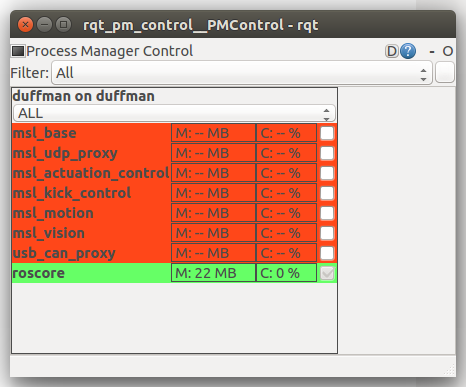
\includegraphics[width=0.6\textwidth]{pic/ProcManRemoteGUI.png}
 \caption{The Remote Controle GUI}
 \label{fig:ProcManRemoteGUI}
\end{figure}

If the process manager and the remote control GUI should run on different PCs, which are in the same network, you need to make sure, that on both machines a roscore and a UDP proxy is running. Therefore, you need to execute the following commands on the machine, where the process manager should run:
\begin{itemize}
 \item \verb#rosrun msl_udp_proxy msl_udp_proxy#
 \item \verb#rosrun process_manager process_manager#
\end{itemize}
The msl-udp-proxy is an autogenerated proxy, which broadcasts MSL specific ROS messages from the local machine to a multicast address on the network. You can also use another UDP proxy (e.g. ttb-udp-proxy, or bbb-udp-proxy), as along as it forwards the \emph{ProcessCommand} and \emph{ProcessStats} ROS messages of the process manager.

On the machine, where the remote control GUI should run, execute:
\begin{itemize}
 \item \verb#roscore#
 \item \verb#rosrun msl_udp_proxy msl_udp_proxy#
 \item \verb#rosrun pm_control pm_control#
\end{itemize}

You need to start the roscore manually, as the remote control GUI does not start a roscore automatically.

\section{General Information on the Process Manager}
\label{sec:GenProcMan}

\subsection*{PROC Filesystem}

The information about the managed processes are collected from the \emph{/proc} filesystem. This is a specific path, which is available on each linux-kernel-based operating system. Inside the /proc folder, each running process has a seperate subfolder, named after its process id (PID). Please note, that this PID is determined by the kernel and has nothing to do with the process ids of the ProcessManaging.conf file. The process manager uses the information available in the processes \emph{cmdline} and \emph{stat} file (e.g. /proc/2341/cmdline). These files are continuesly updated by the kernel. For further information about the proc filesystem, consider chapter 7 of the book \emph{Advanced Linux Programming} (available at: \url{http://www.advancedlinuxprogramming.com/alp-folder/}).

The interesting thing about the proc filessystem approach is, that it enables the process manager to attach to processes it did not start in the first place! If you had some processes already up and running, just start the process manager and its remote control GUI to see the statistics about those processes. 

Another fact about the process manager is, that it does not do anything to the processes, when it is closed. The launched processes are independent of the process manager and continue their execution without it. You accidentally stopped the process manager? No problem just restart the process manager and it will continue to monitor the started processes.

\subsection*{Communication}

The process manager defines two ROS messages: \emph{ProcessCommand} and \emph{ProcessStats}. The ProcessCommand message is used to let him start and stop processes. The ProcessStats message is used by the process manager to report the statistics about its managed processes. The process manager is configured to scan the proc filesystem every two seconds, so that the ProcessStats is send roughly every two seconds.

The process manager subscribes on the ROS topic \emph{/process\_manager/ProcessCommand} and publishes its commands to \emph{/process\_manager/ProcessStats}.

\subsection*{Allowed Number of Processes}

The process manager is written in a way, that it only allows to run a certain process only one time per robot. So if you want to run a process twice on the same machine, you need to modify the \emph{ROBOT} environment variable for at least one of the two process instances. E.g.: \verb#ROBOT=nase rosrun msl_base msl_base -m WM16# and \verb#ROBOT=myo rosrun msl_base msl_base -m WM16#. 

Another feature of the limitation on the number of allowed processes is, that if you did start too many processes, e.g. two or more image processing processes on one robot, you can simply start the process manager and it will clean up the mess. It will kill all but one process of each kind and start reporting statistics about the left processes.

\section{General Information on the Remote Control GUI}
\label{sec:GenRemoteControl GUI}

\subsection*{Process GUI}

The remote control GUI has a single process GUI element for each process (see Figure~\ref{fig:ProcManProcessGUI}). From left to right it shows: the process name, its memory usage in MB, its cpu usage in percent (100\% means one core), its check box for start and stop. The background color of the process GUI is either red (not running), green (running), gray (unknown). Note that the check box does not determine, whether a process is running or not, it is just for starting and stopping a process. Start-Commands for running processes are ignored by the process manager. The check box is disabled for the roscore, because stopping it would cut the communication to the process manager. Check boxes of other processes are disabled too, if they are running with parameters that differ from the currently selected bundle (see~\ref{ssec:BundleSelection}).

\begin{figure}[htbp]
 \centering
 
\includegraphics[width=0.6\textwidth]{pic/ProcManProcessGUI.png}
 \caption{GUI Elements for one Process}
 \label{fig:ProcManProcessGUI}
\end{figure}

If you have a running process (background is green), you can hover over the process GUI element, in order to show its ToolTip. The ToolTip shows the command, which was used to start the process. This way, you don't have to check the ProcessManaging.conf file, in order to know what parameters are used in a certain bundle.


\subsection*{Communication}

The GUI elements are created at runtime, when a corresponding message from a process manager arrives. So if you don't receive any ProcessStats messages, your remote control GUI won't show anything. Furthermore, the GUI elements are deleted, if you don't receive messages for certain amount of time (roughly 3 seconds). The remote control GUI subscribes on the ROS topic \emph{/process\_manager/ProcessStats} and publishes its commands to \emph{/process\_manager/ProcessCommand}.

\subsection*{Bundle Selection}
\label{ssec:BundleSelection}

Selecting a bundle in the drop down box of the GUI, means that the listed processes will be started with the corresponding parameter set, as specified in the ProcessManaging.conf file (see Section~\ref{sec:Configuration}). It also means, that you cannot stop a process which runs with a different parameter set, then specified in the selected bundle. In such cases, the check box of the process is disabled (grayed out). Nevertheless, there are two default bundles: ALL and RUNNING. If you select one of these two bundles, you can interact with all processes.

ALL lists all processes configured in the ProcessManaging.conf file. This is useful, if you want to start a set of processes, which is not specified as an explicit bundle. RUNNING lists all processes of the ProcessManaging.conf file, which are currently up and running. This is useful, for determining, whether there are unwanted processes running, which are not part of the bundle that you would like to use.

\begin{figure}[htbp]
 \centering
 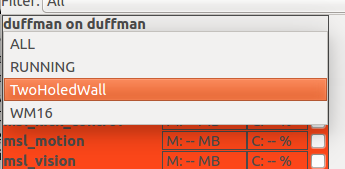
\includegraphics[width=0.4\textwidth]{pic/ProcManBundleSelection.png}
 \caption{Bundle Selection by Drop Down Box}
 \label{fig:ProcManBundleSelection}
\end{figure}

The \emph{roscore} process is specially handled. If the roscore is stopped, the process manager cannot receive commands anymore. Therefore, it is not allowed to stop the roscore process within the remote control GUI.

\section{Configuration}
\label{sec:Configuration}

In order to configure, which processes should be managed by the process manager, you need to edit the \emph{ProcessManaging.conf} file. The file is usually located in the \emph{etc} folder, determined by the \emph{DOMAIN\_CONFIG\_FOLDER} environment variable. Inside the ProcessManaging.conf file several comments explain the config values itself. Nevertheless, lets explain the config for the msl\_base process in detail:

\begin{verbatim}
  [Base]
    id = 7
    execName = msl_base
    rosPackage = msl_base 
    mode = none
    [paramSets]
      1 = -m, TwoHoledWallMaster
      2 = -m, ActuatorTestMaster
      3 = -m, WM16
      4 = -m, TestApproachBallMaster
      5 = -m, TestCheckGoalKicki
      6 = -m, WM16, -sim
    [!paramSets]
  [!Base]
\end{verbatim}

The \textbf{name} (Base) of the outmost section denotes the GUI-String representing the executable. The executable denoted by \textbf{execName} (msl\_base) need to be located in the \emph{PATH} environment variable, or should be found by executing\\ 
\verb#catkin_find --libexec msl_base#\\
in order to work with the process manager. Here \verb#msl_base# is the \textbf{rosPackage} name.

The \textbf{id} of the process must be unique in the ProcessManaging.conf file and is used to refer to this process in the bundles section (explained later) and in the messages send to and received from the process manager.

The \textbf{mode} decides how the process manager handles crashes of the process and some other things. At the moment, there are 3 different modes.
\begin{description}
 \item [none] Basically does nothing. It does not autostart the process, when the process manager is started with the \emph{-autostart} parameter. It does not restart the process, when it did crash.
 \item [keepAlive] Processes, configured with this mode, will be restarted by the process manager, when they crashed.
 \item [autostart] This mode makes the process manager start this process, when the process manager is started with the \emph{-autostart} parameter and restarts it after chrashes.
\end{description}

In the \textbf{paramSets} sections, it is possible to specify different sets of parameters which can be used to start the process. Each parameter set follow a simple key-value-pair convention, where the key must be a (for this process unique) positive integer, greater than 0. The value is a comma (,) seperated list of parameters. Please note, that the parameter \verb#-m TwoHoledWallMaster# is actually two parameters: \verb#-m# and \verb#TwoHoledWallMaster#. The parameter set with the lowest key is considered to be the default parameter set, which means that this parameter set is used, if not specified otherwise (e.g. by choosing a bundle).

The \textbf{bundles} section of the ProcessManaging.conf file allows to specify a set of processes with a specific parameter set for each of it. Here is a small example:

\begin{verbatim}
  [Bundles]
    [WM16]
      processList        = 0,1,2,3,4,5,6,7
      processParamsList  = 0,0,1,0,0,0,0,3
    [!WM16]

    [TwoHoledWall]
      processList        = 0,1,2,3,4,5,6,7
      processParamsList  = 0,0,1,0,0,0,0,1
    [!TwoHoledWall]
  [!Bundles]
\end{verbatim}

In this example, two bundles are specified: WM16 and TwoHoledWall. Each bundle consists of two key-value-pairs: processList and processParamsList. The processList specifies the list of processes, by listing the process ids. The processParamsList specifies the parameter sets for each process. It is important that the order of the processParamsList has to be the same as in the processList. For example: In the WM16 bundle the process with the id 7 (Base) is started with the parameter set id 3 (\verb#-m, WM16#). In the TwoHoledWall bundle, it is started with the parameter set id 1 (\verb#-m, TwoHoledWallMaster#).
The parameter set id 0 is a special value, with the meaning, that there is no parameter set specified for this process, because it has no parameters. 
Another special value, which is only used in the messages send to and received from the process manager, is -1. It says that the parameters of a process are unkown, e.g., the msl\_base is running with an unknown master plan (\verb#-m FancyNewTestPlanMaster#).

\section{Future Work}
\label{sec:ProcManFutureWork}

\begin{itemize}
 \item Make the retry timeout for starting processes a parameter in the ProcessManaging.conf file.
 \item Make it possible to add the GUI for another virtual robot, in order to command a process manager to start processes for another robot. This is necessary for local testing with multiple robots.
 \item Document the implemented feature of starting launch scripts here. (For details see the ProcessManaging.conf file).
\end{itemize}









\chapter{ALICA Client}
\label{chap:ALICAClient}

The ALICA Client is a simple GUI for visualising AlicaEngineInfo messages. Currently it can be started for visualising the messages of a single engine by calling \verb#rosrun alica_client alica_client#. If you have several robots running, the GUI will flicker between their incoming messages. For visualising the messages of multiple robots you should use the Robot Control GUI (see~\ref{chap:RobotControl}). It integrates the same GUI component multiple times.

\begin{figure}[htbp]
 \centering
 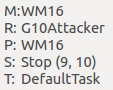
\includegraphics[scale=0.8]{pic/AlicaClient.png}
 \caption{The ALICA Client GUI}
 \label{fig:ALICAClient}
\end{figure}

In Figure~\ref{fig:ALICAClient} you can see the ALICA Client GUI. \textbf{M:} denotes the currently executed master plan (WM16). \textbf{R:} denotes the current role of the robot (G10Attacker). \textbf{P:} is the deepest plan in the alica plan hierarchy, the robot is currently executing. As it is WM16, it means, that it is inside the master plan, but not deeper. Inside this plan, the robot is currently one of two robots inside the Stop state (\textbf{S:}). In this case, it is either the robot with id 9 or 10. The name of the task associated with the active state is the DefaultTask (\textbf{T:}).

This tool is definitely usefull for debugging ALICA plans, but please note, that the AlicaEngineInfo messages are only send roughly every 100ms, but the plan state of an ALICA Engine typically changes much faster, than that. Therefore, you want recognize agents racing through the plans' state machines. Making this visible needs a litte bit more sophisticated GUI, which should be able to read logs of the ALICA engine itself. Please see the \href{http://www.uni-kassel.de/eecs/fileadmin/datas/fb16/Fachgebiete/VS/Documents/ProjectsAndTheses/alica_client.pdf}{project description} for some details, about this possible bachelor project.





\chapter{Robot Control}
\label{chap:RobotControl}

TODO


\chapter{TurtleBot Hardware}
\label{chap:TurtleBotHardware}



\chapter{TurtleBot Software}
\label{chap:TurtleBotSoftware}



\chapter{TurtleBot Gazebo Simulation}
\label{chap:TurtleBotGazeboSimulation}

	
\section{.bashrc}
	\texttt{export TURTLEBOT\_STACKS = ninja-hexagons}
	\\
	\texttt{export TURTLEBOT\_3D\_SENSOR = ninja-kinect}
	\\
	\texttt{export GAZEBO\_MODEL\_PATH}


\section{Starting Gazebo simulation}

\texttt{roslaunch turtlebot\_bringup simulation.launch}
	
	Starts Gazebo, the map server and the robot	
	\\	
	\\	
		
\texttt{roslaunch turtlebot\_bringup navigation\_gazebo.launch}
	
	Starts amcl move\_base
	\\
	\\
	
\texttt{roslaunch rviz\_sim.launch}
	
	Starts local cost map

\section{topics}

\texttt{/leonardo/move\_base\_simple/goal}

	to publish the robots destination
\\
\\
\texttt{/leonardo/initialpose}
	pose estimate	


\section{Turtlebot Sensor Plugin}

To simulate various Scenarios using the Turtlebot there was a need for a more specific and configurable type of sensor. We developed a sensor plugin for gazebo to accomplish that. It allows the user to configure detection angles, range and the type of object in a configuration file. 

\subsection{Configuration}

The configuration format uses a similar syntax as the configuration for the ProcessManager mentioned in a previous section of this document.

The file itself is located at the configuration path (usually \textit{~/ttbws/cnc-turtlebots/etc/}) and has the filename \textit{LogicalCamera.conf}.

Let's take a look at the following example configuration:

\begin{verbatim}
[LogicalCamera]
        [Victim]
                # meter
                range = 3
                type = victim
                # Hz
                publishingRateHz = 1

                # angles have to be set from 180 to -180 degree
                [DetectAngles]
                        [Front]
                                startAngle = -135
                                endAngle = 135
                        [!Front]
                [!DetectAngles]
        [!Victim]
        [Fire]
                # meter
                range = 5
                type = fire
                # Hz
                publishingRateHz = 10

                # angles have to be set from 180 to -180 degree
                [DetectAngles]
                        [Front]
                                startAngle = -180
                                endAngle = 180
                        [!Front]
                [!DetectAngles]
        [!Fire]
[!LogicalCamera]
\end{verbatim}

The first Block \texttt{[LogicalCamera]} is the uppermost block and has to be followed by \texttt{[!LogicalCamera]} at the end.

In this example we want to detect two types of objects. The first one is the presence of victims and the second one is fire. Each distinct type has to be defined as a block, similar to the uppermost LogicalCamera Block. Hence we have \texttt{[Victim] ... [!Victim]} and \texttt{[Fire] ... [!Fire]} here.

In these type blocks, we now have to define the properties of the sensor for that given type of object.

Here, a victim can be detected in a \textbf{range} of 3 meters, as given to  the range parameter.

The \textbf{type} parameter is used by the plugin to determine which object belongs to which type. The plugin filters these types depending on the objects name in gazebo. So an object called \textit{victim\_box} is going to be detected as a victim type object.

Using the parameter \textbf{publishingRateHz} as the name suggests you can set the rate in which an object may be detected. A victim will be only detected once a second, while a fire can be detected up to ten times a second.

Next, the block \textbf{DetectAngles} allows you to specify multiple sections in which the robot can detect the object.

Anlges have to be in a range from -180° to 180°.

The following picture clarifies, how the angles have to be speciefied:

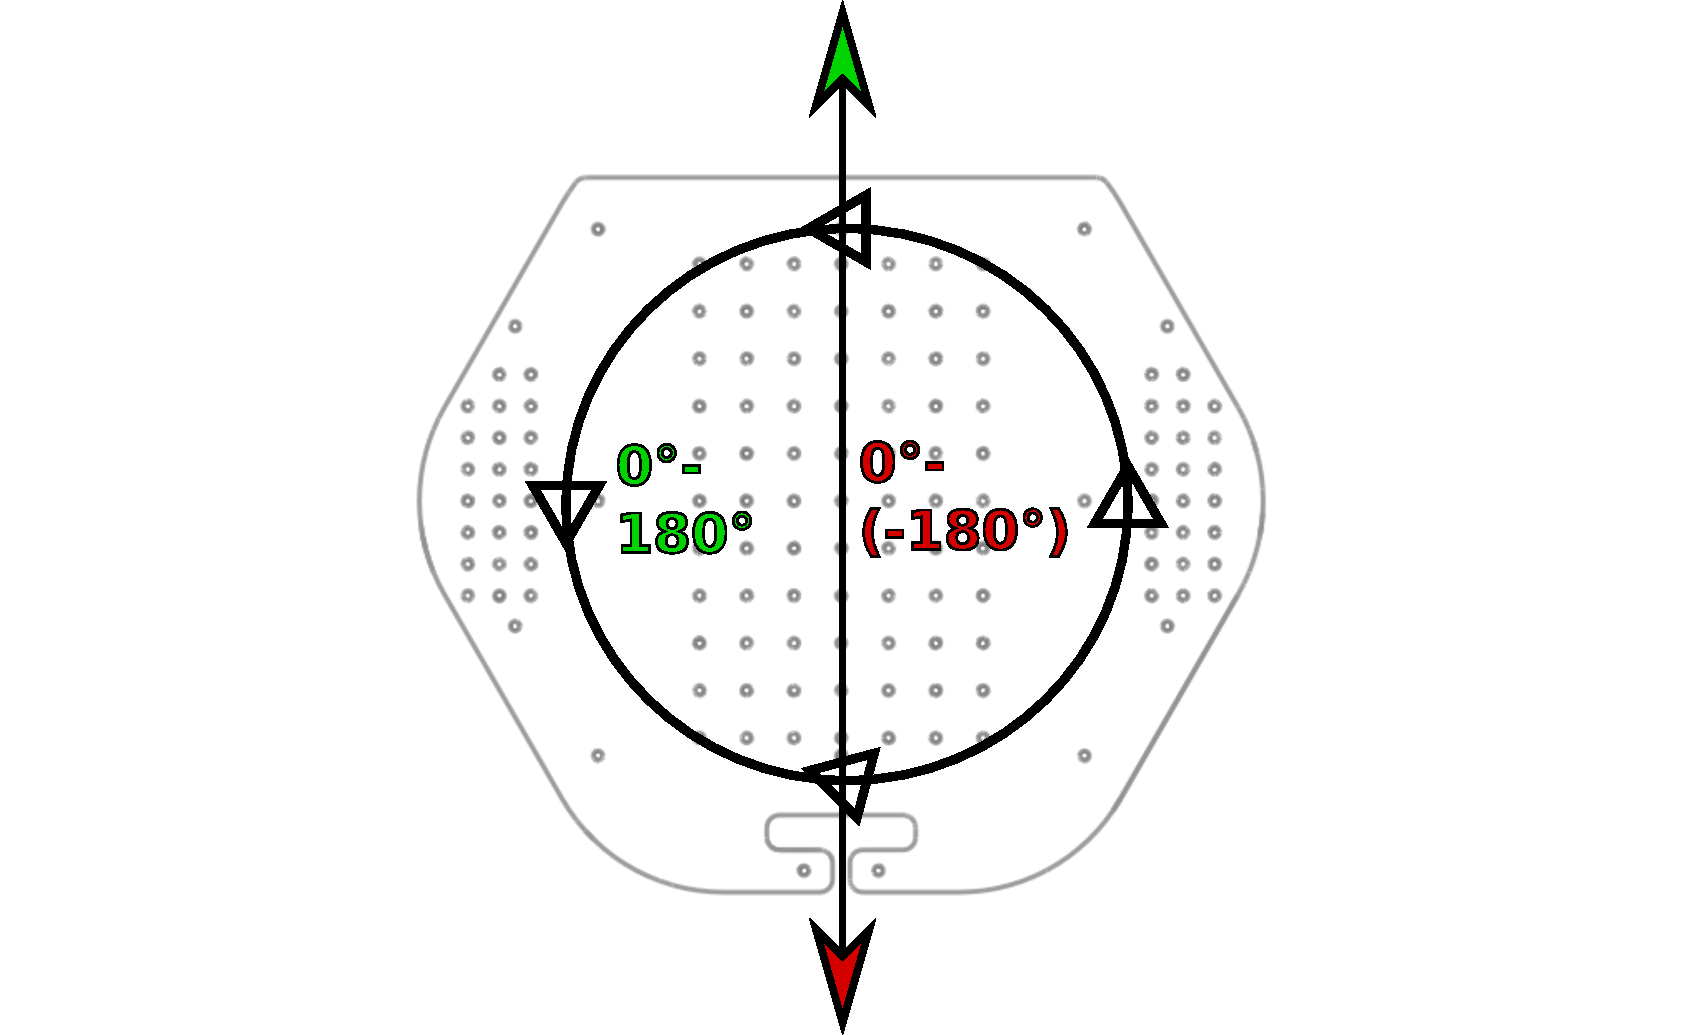
\includegraphics[width=1.0\textwidth]{ttbangles.pdf}

\subsection{Sensor message}

Every time an object has been detected according to the configuration, a ROS message gets sent.

The name of the ros topic is \textit{logical\_camera} and is namespaced with the robot name, as configured in the \textit{robot.simulation} file. So for a robot named leonardo, the message will get published on the topic  /leonardo/logical\_camera.\\

The message itself has the following fields:

\texttt{string modelName}

	Name of the detected model/object in gazebo

\texttt{geometry\_msgs/Pose2D pose}

	Posoition of the object on the x,y plane(map seen from top)

\texttt{ObjectSize size}

	Approximate size of an object. Contains fields xsize, ysize and zsize.

\texttt{time timeStamp}

	Time, when the object was detected.

\texttt{string type}

	Object type. See Configuration Section for details.

\newpage
\subsection{Robot coordinate system}

Looking from the top at the turtlebot, the coordinate system looks like that:

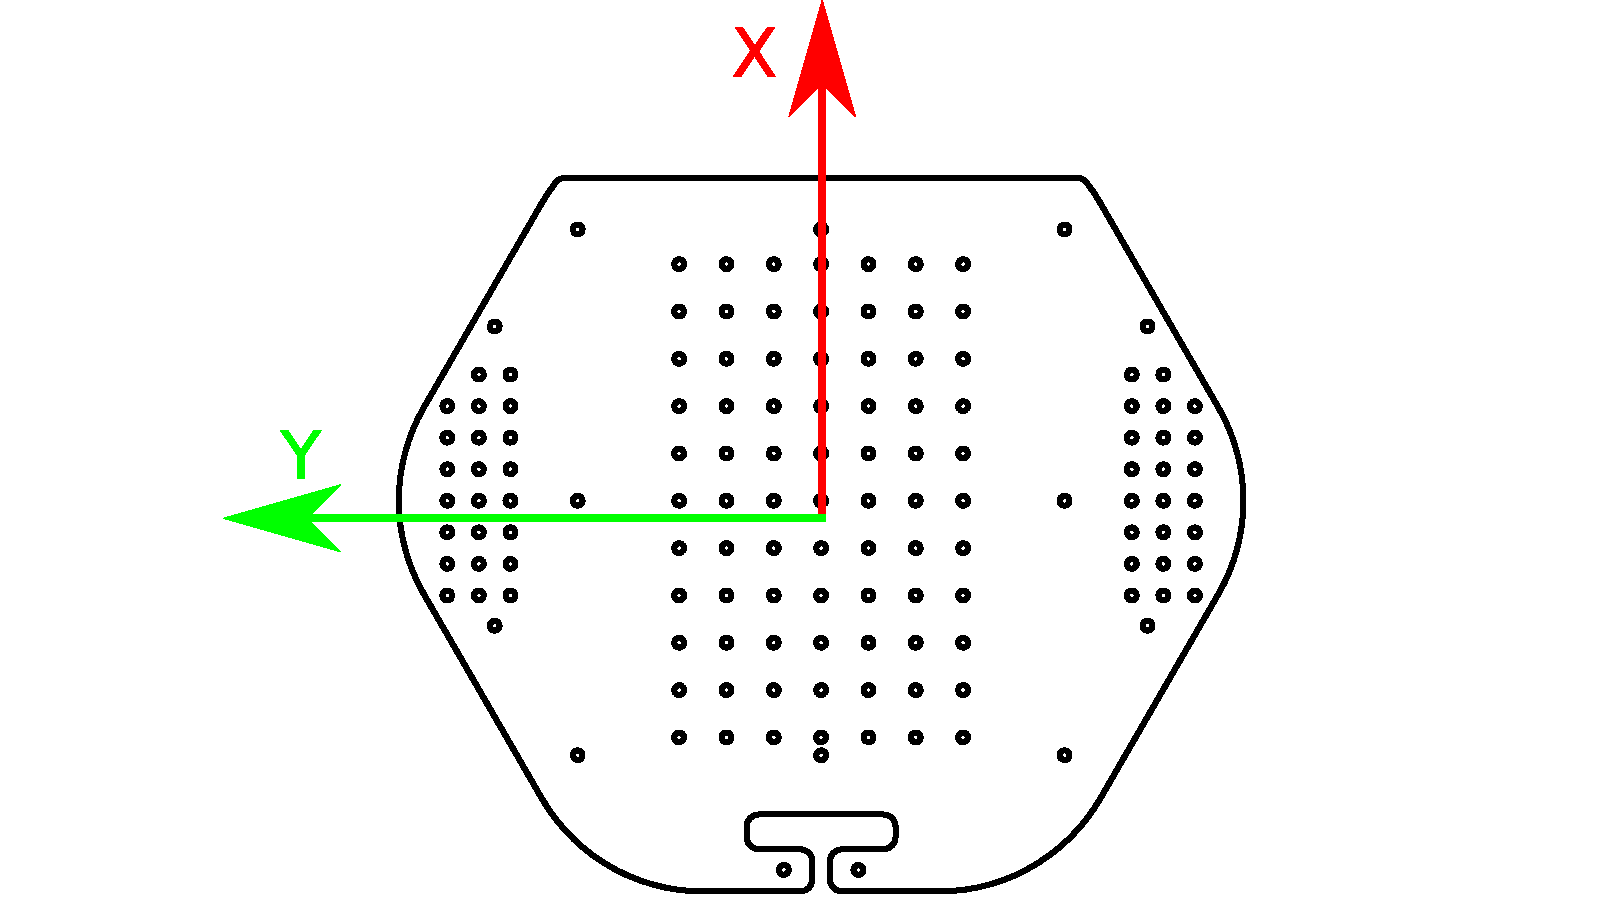
\includegraphics[width=1.0\textwidth]{ttbtop.pdf}

So the a positive X coordinate means, an object is ahead of the robot, while a negative one means, it is behind the robot. In the same way, a positive Y means that an object is detected left of the robot, while a positive Y coordinate means that it was detected on the right side.

As a side note, the Z coordinate tells you how high is an object in relation to the sensor. A positive Z means, that the object is above the sensor, while a negative Z means, that it is negative.

\subsection{Using the sensor plugin in gazebo}

First, make sure you configured the plugin as described in the configuration section.

Then simply launch gazebo using the simulation launch file:

\begin{verbatim}
roslaunch turtlebot_bringup simulation.launch
\end{verbatim}

In order for the plugin to correctly detect and filter the objects, you have to give each object a name, that contains the type string from the configuration. A \textit{victim\_box} may for example be detected  as a victim or box type of object.

Now, to add objects in Gazebo you can for example add a cube using the cube button in toolbar on top of the 3D view. For more information about adding objects in gazebo, take a look at the corresponding gazebo tutorial.

To quickly test the sensor you can add a cube or sphere and rename it as follows.  First, add an object using the cube, sphere or cylindar button in the top bar. Then select the object by left clicking on it and then right click it to bring up the context menu. In the menu select \textit{Edit Model}. You are now in the Model Editor. In the left Pane select the Model Tab and change the Model Name to a name that contains the type string. After you are done, exit the Model Editor by select \textit{Exit Model Editor} in the \textit{File Menu}.

Now you may have to continue the simulation by pressing the play button on the bar below the 3D view. After that you should be able to receive messages from the plugin on the \textit{logical\_camera} topic.

\appendix
\chapter{Appendix}
\label{chap:Appendix}

\begin{landscape}
  \section{.bashrc}
  \label{sec:bashrc}
  \begin{figure}[htbp]
    \begin{verbatim}
# ROS specific 
source /opt/ros/melodic/setup.bash

# TurtleBots
ttbws_path=<insert your path to the ttbws folder here>

source ${ttbws_path}/devel/setup.bash

# ALICA/ttb_base specific stuff
export DOMAIN_FOLDER=${ttbws_path}/src/cnc-turtlebots/
export DOMAIN_CONFIG_FOLDER=${DOMAIN_FOLDER}/etc

# for loading the right models (environment and robot)
export GAZEBO_MODEL_PATH=${GAZEBO_MODEL_PATH}:${ttbws_path}/src/turtlebot/turtlebot_bringup/models
export TURTLEBOT_STACKS=ninja-hexagons
export TURTLEBOT_3D_SENSOR=ninja-kinect

#fancy prompt that also shows the current git branch
export PS1='\[\033[01;32m\]\u@\h\[\033[01;34m\] \w \[\033[01;31m\]$(__git_ps1 "[%s]")\[\033[01;34m\]\$\[\033[00m\] '
    \end{verbatim}
    \caption{Template for your .bashrc}
    \label{fig:template_bashrc}
  \end{figure}
\end{landscape}

\chapter{Exam}
\label{chap:Exam}

The question in all courses is: ``What is relevant for the exam?''

Each semester I will try to give an answer to that question again and again \ldots and again. \textbf{Here is my answer (not fixed yet) for the winter term 2016/17}:

You should be able to give the right answer to the following questions and be able to fullfil the given tasks:

\section{Questions: Foundations}
\label{sec:questions_foundations}

\begin{itemize}
 \item What is an agent?
 \item What is an autonomous agent?
 \item Sketch a state-of-the-art robot control architecture and explain its components.
 \item What is the difference between trueness and precision?
 \item Name two different sensors and explain their categories, properties, and value properties.
 \item What is an actuator?
 \item What is odometry?
\end{itemize}

\section{Questions: External Software and Developing Tools}
\label{sec:questions_tools}

\begin{itemize}
 \item What is a version control system and what is it good for?
 \item What does git pull, push, commit, etc. do?
 \item What is ROS and what is it good for?
 \item Describe the publish-subscribe model for communication.
 \item Describe the notion of nodes, topics, messages, publishers, subscribers.
 \item What is a Build Chain?
 \item What is CMake and for what do we use it?
\end{itemize}

\section{Questions: C++}
\label{sec:questions_c++}

\begin{itemize}
 \item What is written in the header file and what in the source file of a C++ class?
 \item How does a shared\_ptr work and what is it good for?
 \item Explain roughly what the gcc compiler does.
\end{itemize}

\section{Questions: Real Robots}
\label{sec:questions_robots}

\begin{itemize}
 \item Which sensors does the TurtleBot have and what are they good for?
 \item Explain the details of the laser scanners sensor properties.
 \item Why do we use the extra laser scanner on the TurtleBot?
\end{itemize}

\section{Questions: Gazebo Simulation}
\label{sec:questions_simulation}

\begin{itemize}
 \item Why do we use the logical camera sensor in simulation?
\end{itemize}

\section{Questions: Navigation and Mapping}
\label{sec:questions_nav_and_map}

\begin{itemize}
 \item What is a CostMap?
 \item Explain the following diagram (see Figure~\ref{fig:costmap}).
 \item Sketch the CostMap on the following drawing.
 \item Sketch an algorithm for driving to the given destination (see Figure~\ref{nav_task}) with the help of the laser scanner data.
 \item Denote the input and the output of AMCL and sketch how AMCL is calculating the robtos position based on the input.
\end{itemize}

\begin{figure*}[htbp]
 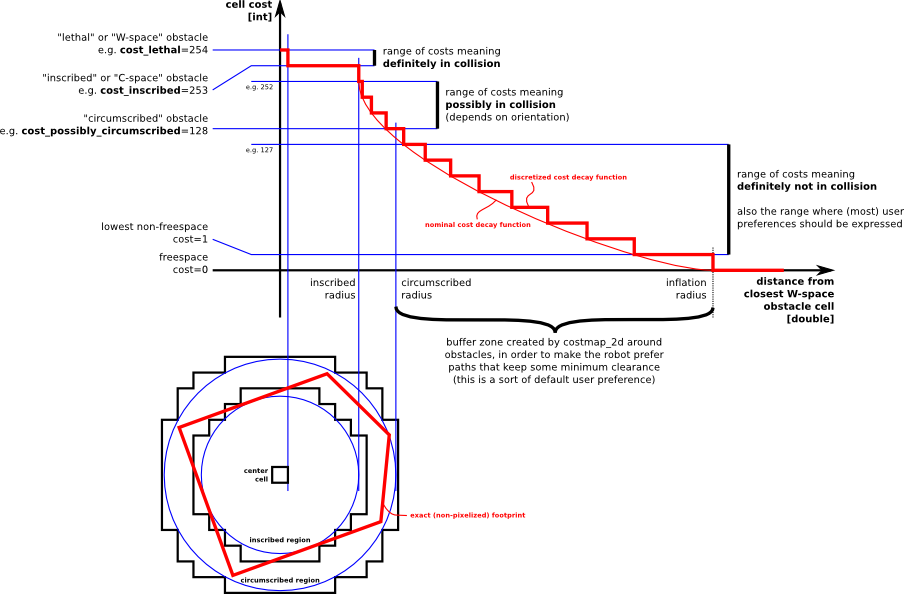
\includegraphics[width=\textwidth]{pic/costmapspec.png}
 \caption{CostMap Valuation Diagram (Source: http://wiki.ros.org/costmap\_2d)}
 \label{fig:costmap}
\end{figure*}

\begin{figure*}[htbp]
 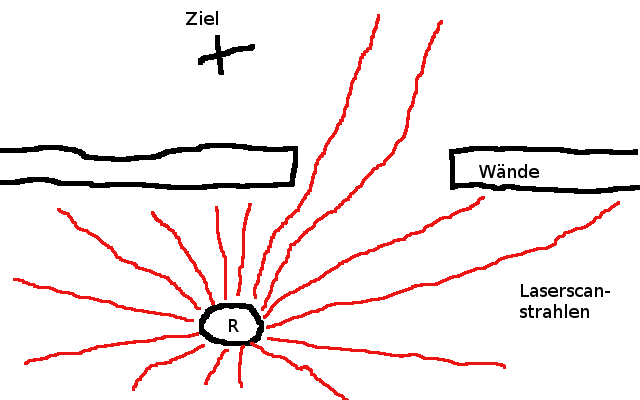
\includegraphics[width=\textwidth]{pic/simple_nav.png}
 \caption{A Simple Navigation Task}
 \label{fig:nav_task}
\end{figure*}


\section{Questions: Application Scenario}
\label{sec:questions_app_scenario}

\begin{itemize}
 \item For what is the ARTracker module?
 \item How is it possible that two TurtleBots communicate about positions, without having a common map?
 \item For what did we use the laser scanner?
\end{itemize}




% CONFIGURE BIBLIOGRAPHY PENALTIES
\setcounter{biburlnumpenalty}{9000}
\setcounter{biburlucpenalty}{9000}
\setcounter{biburllcpenalty}{9000}

% BIBLIOGRAPHY
\printbibliography

\end{document}
